\def\mytitle{\textbf{ASSEMBLY ASSIGNMENT}}
\documentclass[10pt,a4paper]{article}
\usepackage[a4paper,outer=1.5cm,inner=1.5cm,top=2cm,bottom=1.5cm]{geometry}
\usepackage{listings}
\usepackage{circuitikz}
\usepackage{titlesec}
\usepackage[utf8]{inputenc}
\usepackage{amsmath}
\usepackage{graphicx}
\usepackage{amsfonts}
\usepackage{textgreek}
\usepackage{tabularx}
\title{\mytitle}
\author{Pavan Srinivas Marri\\marripavan65@gmail.com\\FWC22138 IITH - Future Wireless Communications}
\date{}
\begin{document}
\maketitle
\graphicspath{{./Documents}{./figs}}
\tableofcontents
	\section{Problem}
	(GATE2019-QP-EE)\\
		Q.36 In the circuit shown below , X and Y are digital inputs, and Z is a digital output. The equivalent circuit is a
		\begin{figure}[h!]
	     	\begin{center}
		\centering
		\begin{circuitikz}[scale=1]
    % 1st not
        \draw (0,0) node[not port,scale=0.8 ] (not) {};
        \draw (3,-0.28) node[and port] (and) {};
        
        \draw (not.in 1) -- ++(-1,0) node[left] {$X$};
        \draw (not.out) -- ++(0,0) coordinate (and.in 1);
        \draw (not.in 1) -- ++(0,-1.7) node[below] {$ $};
    % 1st And
        \draw (and.in 1) -- ++(-1.2,0) node[left] {$ $};
        \draw (and.in 2) -- ++(-3.3,0) node[left] {$Y$};
        \draw (and.out) -- ++(0,0) node[right] {$ $};

        \draw (and.in 2) -- ++(-3,0) coordinate (point);
        \draw (point) -- ++(0,-1.7) -- ++(1,0) node[below] {$ $};
        \draw (and.out) -- ++(0,-0.47) node[below] {$ $};
    %2nd not
        \draw (0,-2.28) node[not port ,scale=0.8] (not) {};
        \draw (not.in 1) -- ++(-0.8,0) node[left] {$ $};
        \draw (not.out) -- ++(0,0) coordinate (and.in 2);
   %2nd ANd
        \draw (3,-2) node[and port] (and) {};
        \draw (and.in 1) -- ++(-2.2,0) node[left] {$ $} ;
        \draw (and.in 2) -- ++(-1.2,0) node[left] {$ $} ;
        \draw (and.out) -- ++(0,0) node[right] {$ $};
          \draw (and.out) -- ++(0,0.7) node[above] {$ $};
    %or
        \draw (6,-1) node[or port] (or) {};
        \draw (or.in 1) -- ++(-1.48,0) node[left] {$ $} ;
        \draw (or.in 2) -- ++(-1.48,0) node[left] {$ $} ;
        \draw (or.out) -- ++(1,0) node[right] {$Z$};
  
     \end{circuitikz}
		\end{center} 
		\end{figure}
			\begin{enumerate}
				\item[(A)] NAND gate
				\item[(B)] NOR gate
				\item[(C)] XOR gate
				\item[(D)] XNOR gate
			\end{enumerate}

	\section{Components}
		\begin{table}[htbp]
		\centering
			\begin{tabularx}{1\textwidth}
			{
				| >{\centering\arraybackslash}X
				| >{\centering\arraybackslash}X
				| >{\centering\arraybackslash}X |}
			\hline
			{\bf Components} & {\bf Value} & {\bf Quantity} \\
			\hline
			Arduino & Uno & 1\\
			\hline
			BreadBoard & &  1 \\
			\hline
			Jumper Wires & & 4 \\
			\hline
		\end{tabularx}
			\caption{Components}
			\label{table=Components}
		\end{table}

	\section{Implementation}
				\subsection{Boolean Expression}
 				By solving above expression we get :
				\begin{align}
					z=& x' . y +x.y' \nonumber \\
					z=& x'y+xy' \nonumber  \end{align} 
			\subsection{Truth Table}

                        \begin{table}[htbp] 
				\centering  
				\begin{tabularx}{0.5\textwidth}
                        {  | >{\centering\arraybackslash}X
                           | >{\centering\arraybackslash}X
                           | >{\centering\arraybackslash}X |}
                         \hline
                         {\bf A} & {\bf B} & {\bf OUT} \\
                       \hline 
			0 & 0 & 0\\   
			\hline  
			0 & 1 & 1 \\
                       \hline                                                                                                             
	         	1 & 0 & 1 \\  
		        \hline   
			1 & 1 & 0 \\
			\hline
			\end{tabularx}
                        \caption{Truth Table}
				\label{table=truth}
			\end{table}
     \section{Hardware}
	     \begin{enumerate}
		     \item Make the connections between the arduino and Breadboard as shown in Table3.
			     \begin{table}[h]
				     \centering
				     \begin{tabularx}{0.5\textwidth}
					     {
						     | >{\centering\arraybackslash}X
						     | >{\centering\arraybackslash}X
						     | >{\centering\arraybackslash}X |}
						     \hline
						     {\bf Arduino} & 5.0v & GND \\
						     \hline
						     {\bf Breadboard} & +ve & -ve  \\
						     \hline
				     \end{tabularx}
				     \caption{\label{Table-3}Connections}
			     \end{table}
			     \item Connect one end of a jumper wire to the GND(ground) pin on the Arduino Uno board and other end to the 
				     breadboard’s ground rail(-).
                             \item Connect one terminal of jumper wire (Input A) to the input pins on the Arduino(e.g., pin2) and other terminal to
				     the positive rail(+) on the breadboard.
			     \item Connect one end of another jumper wire (Input B) to the input pin of Arduino(e.g., pin3) and other end to the 
				     positive rail(+) on the breadboard.
			     \item Enable the power supply to breadboard from arduino by connecting one end of jumper wire to the power pin of
				     Arduino(5V) and other end to the positive rail(+) on the breadboard.
			     
	     \end{enumerate}
	     \begin{figure}[h!]
		     \centering
		     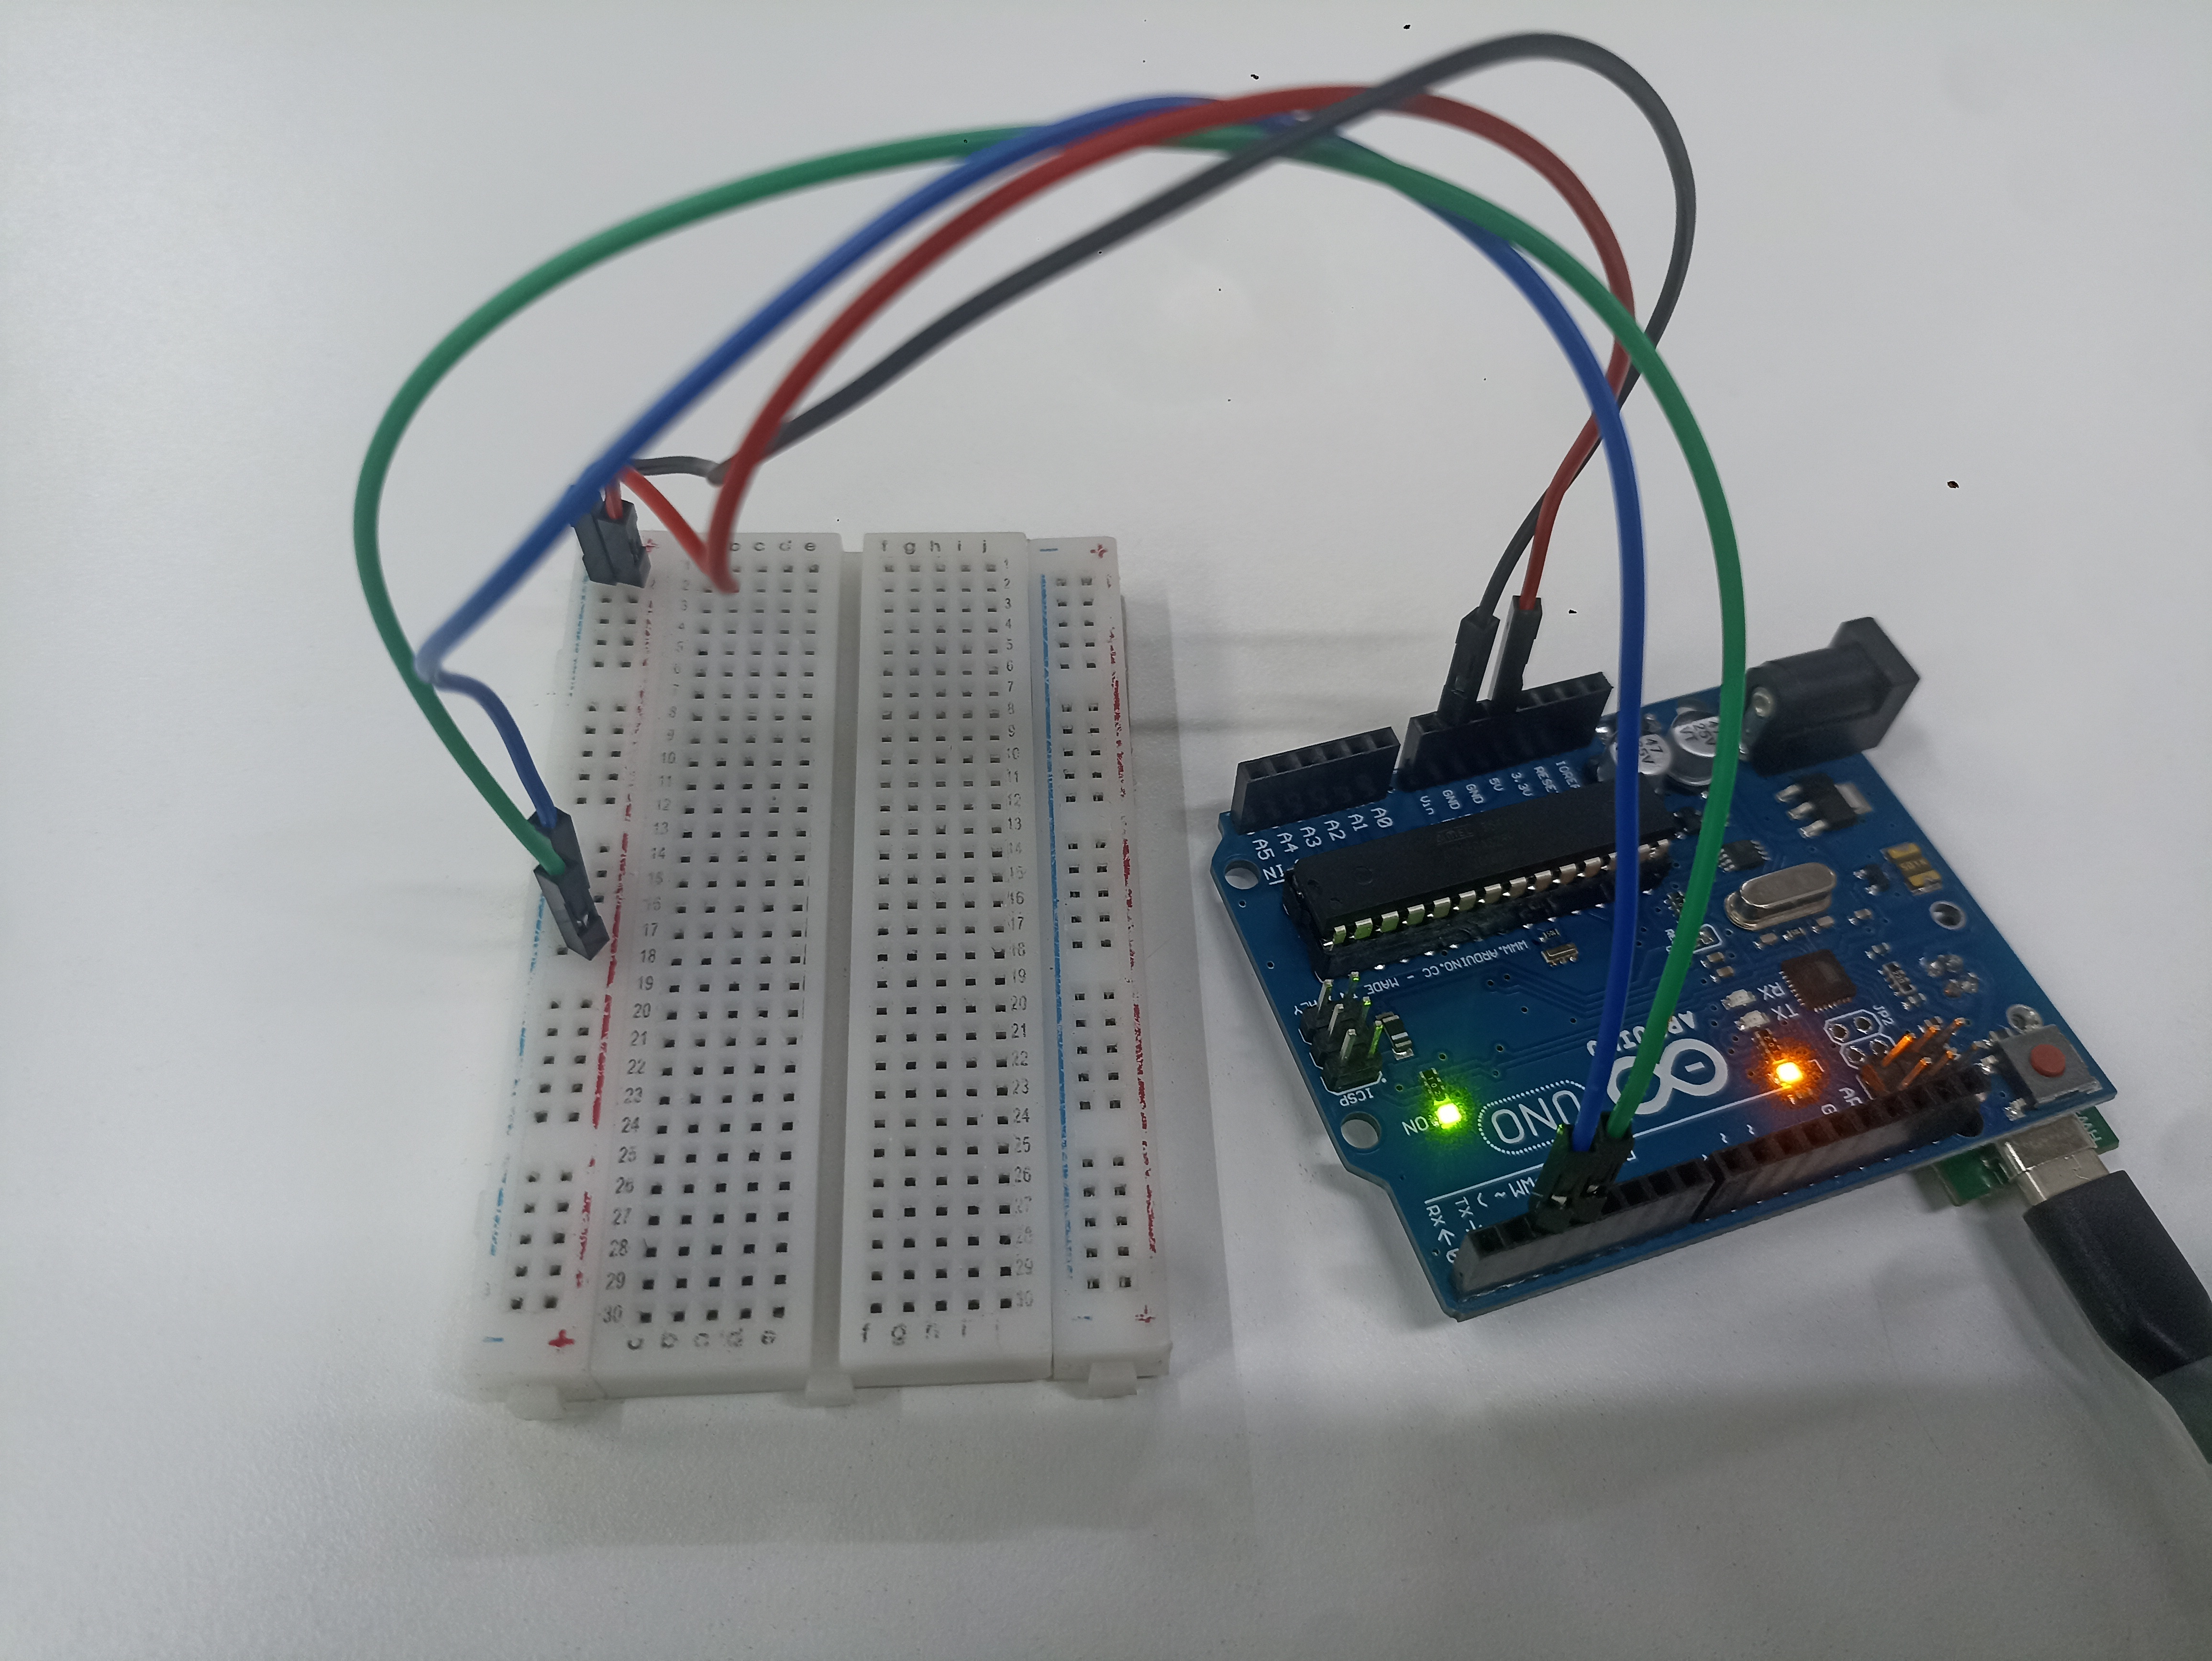
\includegraphics[width=0.3\columnwidth]{assembly.jpg}
		     \caption{Connections}
		     \label{fig:connections}
	     \end{figure}
     \section{Software}
	     Now write the code which is available in below path and upload to the Arduino.\\
	     \framebox{https://github.com/Pavan2k01/Digital-Design/tree/main/Assembly/Assembly.asm}
	     \section{Conclusion}
	     Hence, we have implemented the XOR gate for the given circuit using the code in Assembly language with the help of Arduino.
\end{document}
